\documentclass[12pt]{report}

\usepackage{subfigure}
\usepackage[english]{babel}
\usepackage[utf8x]{inputenc}
\usepackage[T1]{fontenc}

\usepackage{graphicx}
\usepackage{float}
\usepackage{pgfgantt}   
\usepackage{lipsum}
\usepackage{graphicx}
\usepackage{natbib}
\usepackage{setspace}

%% Sets page size and margins
\usepackage[a4paper,top=3cm,bottom=3cm,left=3cm,right=3cm,marginparwidth=1.75cm]{geometry}

%% Useful packages
\usepackage{amsmath}
\usepackage{graphicx}
\usepackage[colorinlistoftodos]{todonotes}
\usepackage[colorlinks=true, allcolors=black]{hyperref}

\begin{document}
\begin{titlepage}
    % \newgeometry{top=25mm,bottom=25mm,left=38mm,right=32mm}
    \setlength{\parindent}{0pt}
    \setlength{\parskip}{0pt}
    % \fontfamily{phv}\selectfont
    
    {
                    \Large
                    \raggedright
                    Imperial College London\\[17pt]
                    Department of Electrical and Electronic Engineering\\[17pt]
                    Final Year Project Report 2019\\[17pt]
    
    }
    
    \rule{\columnwidth}{3pt}
    \vfill
    \centering
      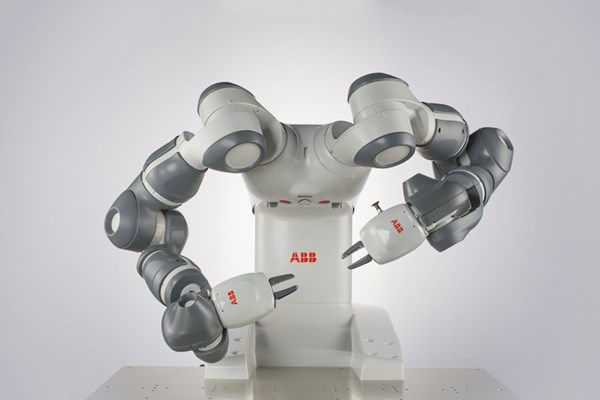
\includegraphics[width=\columnwidth,height=80mm,keepaspectratio]{title/YuMicover.jpeg}
    \vfill
    \setlength{\tabcolsep}{0pt}
    
    \begin{tabular}{p{40mm}p{\dimexpr\columnwidth-40mm}}
                    Project Title: & \textbf{Robot Manipulation of Shoe Laces -- AI Planning and Control} \\[12pt]
                    Student: & \textbf{Zengyang Pan} \\[12pt]
                    CID: & \textbf{01046157} \\[12pt]
                    Course: & \textbf{4EM} \\[12pt]
                    Project Supervisor: & \textbf{Prof Yiannis Demiris} \\[12pt]
                    Second Marker: & \textbf{Dr Tae-Kyun Kim} \\
    \end{tabular}
\end{titlepage}

\onehalfspacing
\setlength{\parskip}{0.5em}
\begin{abstract}
%The abstract is a very brief summary of the report’s contents. Somebody unfamiliar with your project should have a good idea of what it’s about having read the abstract alone and will know whether it will be of interest to them. The abstract should (very concisely) summarise the topic, content and conclusions of the project. Abstracts can vary in length from 50 words up to at most 200 words. They are more concise than executive summaries.

This project

%This report reviews work on motion planning and object detection, examines available vision and robotic hardware for performing shoe lace and hole detection and manipulation, and establishes the criteria for the middleware that will be used for the project. Evaluation criteria are established as a sequence of increasingly difficult shoelace manipulation, starting from passing through a shoe hole, up to fully completing a shoe.
\end{abstract}

\renewcommand{\abstractname}{Acknowledgements}
% It is usual to thank those individuals who have provided particularly useful assistance, technical or otherwise, during your project. 
\begin{abstract}
Thanks mum!
\end{abstract}

%\hypersetup{linkcolor=black}
\setlength{\parskip}{0em}
\tableofcontents
\newpage

%\listoffigures
%\listoftables
\setlength{\parskip}{0.5em}
\chapter{Introduction}
%It should begin with a clear statement of what the project is about so that the nature and scope of the project can be understood by a lay reader. 

In the past decades, robots have become an indispensable role in human life. There are various types of robots in the fields of manufacturing, healthcare, education, entertainment and military etc. No matter which category a robot belongs to, it is essential to endow the robot with some abilities so that it can perform corresponding tasks. Currently, there are mainly three approaches to teach skills to robots: direct programming, imitation learning and reinforcement learning, according to \citep{Kormushev_MDPI_2013}. However, there exists a trade-off between the difficulty to teach and computational complexity. Thus, a different approach should be adopted based on task specification.

\section{Motivation}
Speaking of non-industry environments, robot manipulation tasks usually cannot rely on hard-coded knowledge about the scene structure. This is because the environment can be modified by human actions, which is unforeseeable. Thus, a vision-based object recognition and localization system is extremely useful for providing the robot with scene knowledge. By combining computer vision techniques with motion planning, it enables robots to perform tasks more flexible and equip with a certain degree of autonomy.

\section{Objectives}
%ability independently to formulate and solve technical problems in project work. 
%project is intended to deliver, hardware, software, simulation, and analytical work.
Therefore, as my final year project, I aim to develop an algorithm for a bi-manual robot so that it can put shoelace on a shoe. In the core project, starting with one arm holding one end of the shoelace, the robot should detect a shoe hole and plan an arm trajectory to pass the shoelace through that hole. As an extension, the robot should be able to plan sequences of trajectories in order to complete the whole shoe.

\section{Challenges}
Due to the relatively small size of the shoe hole, this project requires a high degree of precision. Firstly, the optimal methods to localize the shoe hole need to be figured out. Then, the main challenge is to calculate the direction in which the lace should pass through the shoe hole in the dynamic environment. In addition, how to use robot arms to achieve this task accordingly also requires an accurate analysis. Finally, plenty of tests regarding the whole system need to be done in order to optimize the performance.

\section{Report Structure}
This report is structured as follows:

\begin{itemize}
    \item \textbf{Chapter 2 - Background} provides a background analysis of this project, including the choice of robot and camera, possible implementation approaches for both motion planning and computer vision side, as well as the chosen operating system and software. 
    \item \textbf{Chapter 3 - Requirement Capture} describes the detailed deliverables of the core project and extension, so that the reader can keep the objectives in mind while reading the remaining part.
    \item \textbf{Chapter 4 - Analysis and Design} introduces the designed system overview and workflow in order to achieve both the core project and extension. A brief introduction to the operating system and the robot status is included as well.
    \item \textbf{Chapter 5 and 6 - Implementation} gives the detailed approaches to fulfill the project requirements.
    \item \textbf{Chapter 7 - Testing and Results} presents a series of experimental results of the implemented methods. Success rate and execution time are the two evaluation criteria.
    \item \textbf{Chapter 8 - Conclusion} summarises the achievements of this project together with the advantages and limits. 
    \item \textbf{Chapter 9 - Future Work} suggests a few extra implementation ideas that could extend the scope of this project. 
    \item \textbf{Chapter 10 - User Guide} offers the instructions to launch this project.
\end{itemize}

\chapter{Background}
%Thorough discovery of background material. Decisions made in the project are correctly informed by background. Analysis of competing products, software standards, necessary software tools, background theory.
% The background section of the report should set the project into context by relating it to existing published work which you read at the start of the project when your approach and methods were being considered. The published work may be in the form of research papers, articles, text books, technical manuals, or even existing software or hardware of which you have had hands-on experience.

%link (and make explicit this link between) the different topics in a coherent pipeline: hardware-(choice of robot) > motion planning->state information (camera) (object detection +  orientation detection)-> etc
This chapter contains background information about this project. Several potential implementation approaches are discussed, and the design choices are made. As illustrated in Figure \ref{bgov}, the content starts with robot selection, then dives into motion planning algorithms. The available cameras that provide state information for the robot are then evaluated and chosen. After that, the techniques for objects 6D pose calculation are summarised and compared, which consists of object detection and orientation estimation. Finally, the system and software used to implement the selected methods are introduced.

\begin{figure}[H]
\centering
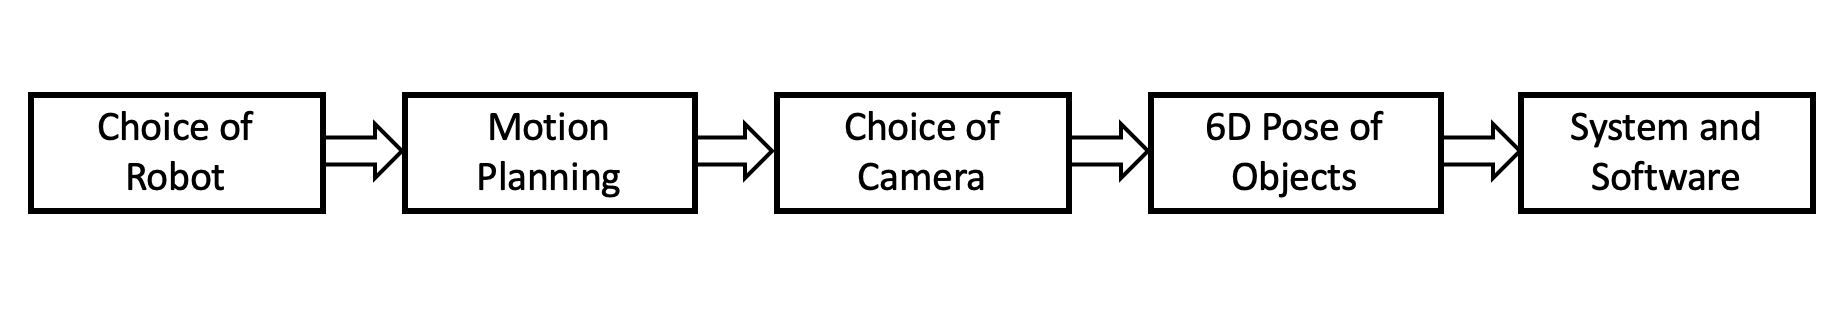
\includegraphics[width = \columnwidth]{background/backgroundov.png}
\caption{The order of background introduction}
\label{bgov}
\end{figure}

\section{Choice of Robot}
There are three robots available for this project: iCub, Baxter and ABB YuMi.

The \citep{iCub} is a 1-metre tall humanoid robot for research in human cognition and artificial intelligence, which has 53 actuated degrees of freedom across its body. Moreover, it has facial expressions and can establish eye contact with users. However, its joints are relatively weaker than Baxter and YuMi. Considering this project only needs vision and robot arms, iCub is not considered as the best robot.

\begin{figure}[H]
\centering
\subfigure[iCub]{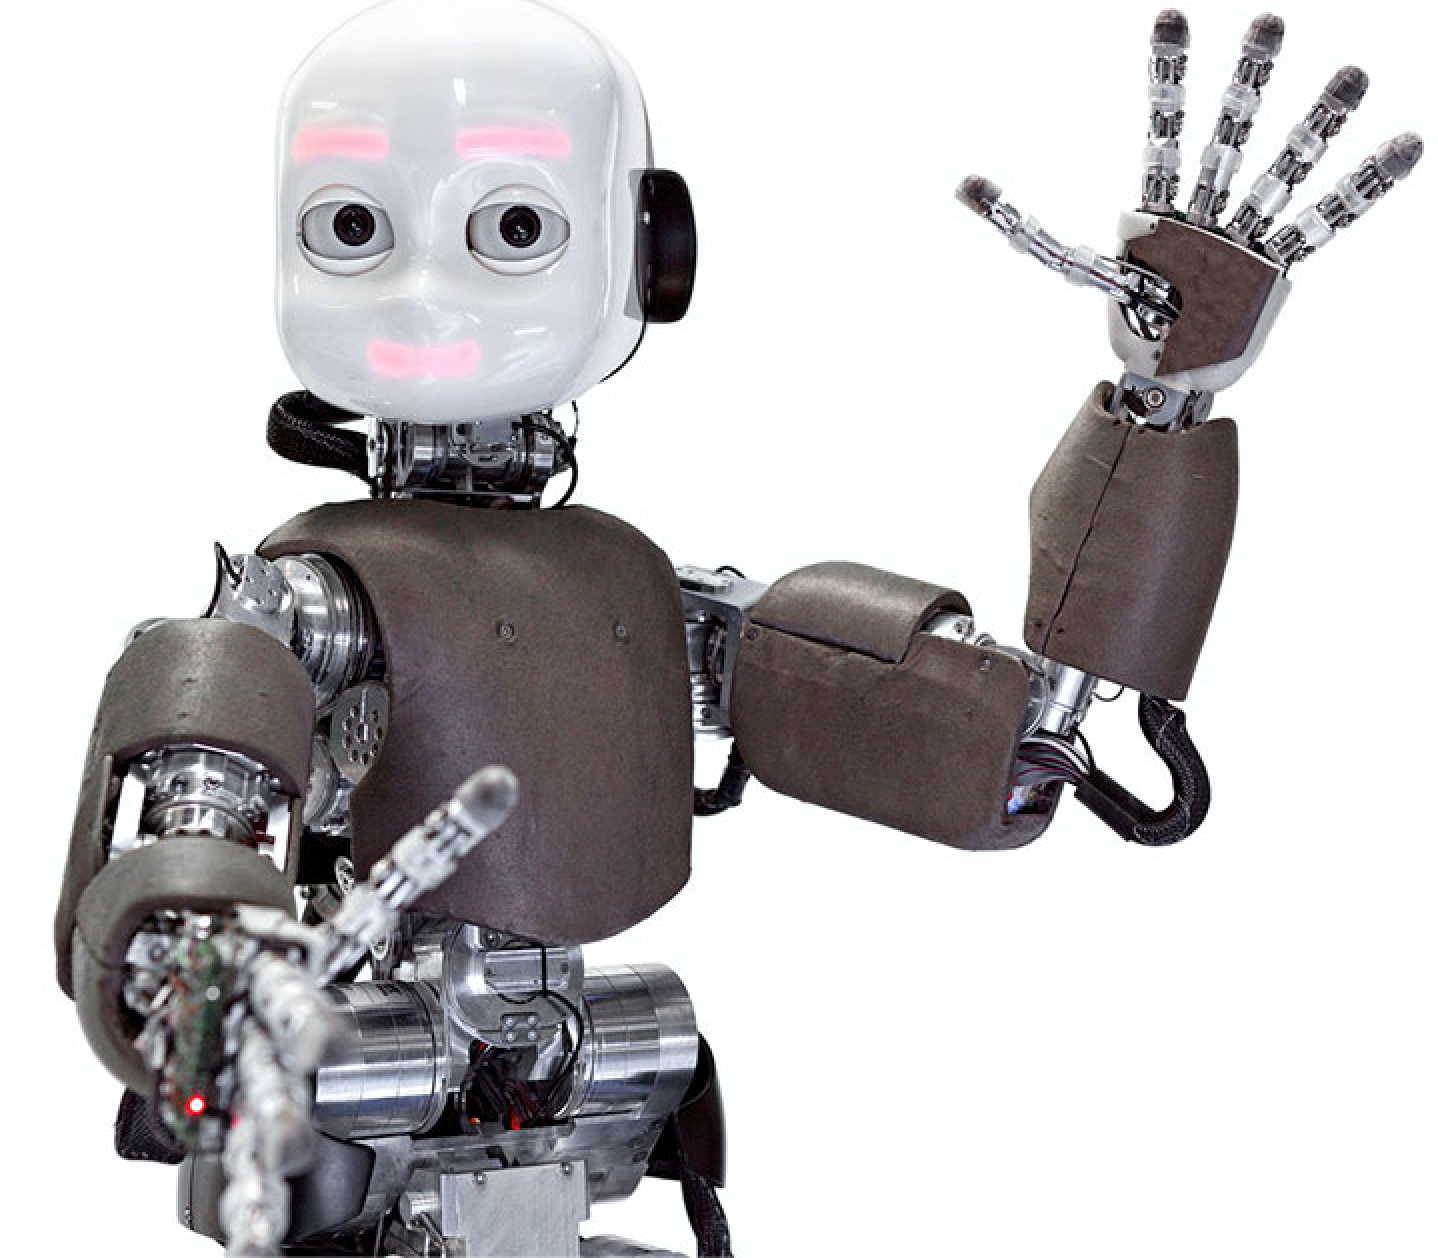
\includegraphics[width = 0.32\columnwidth]{background/icub.png}}
\subfigure[Baxter]{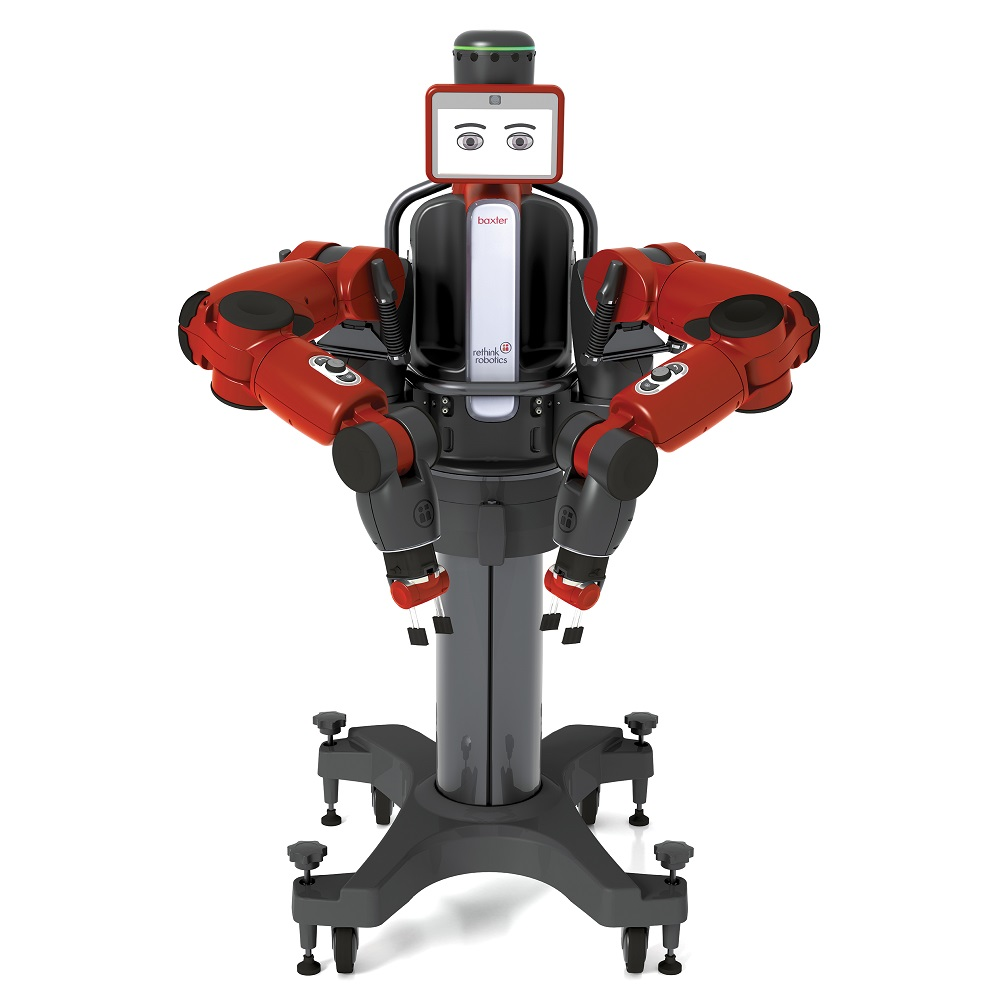
\includegraphics[width = 0.32\columnwidth]{background/baxter.png}}
\subfigure[ABB YuMi]{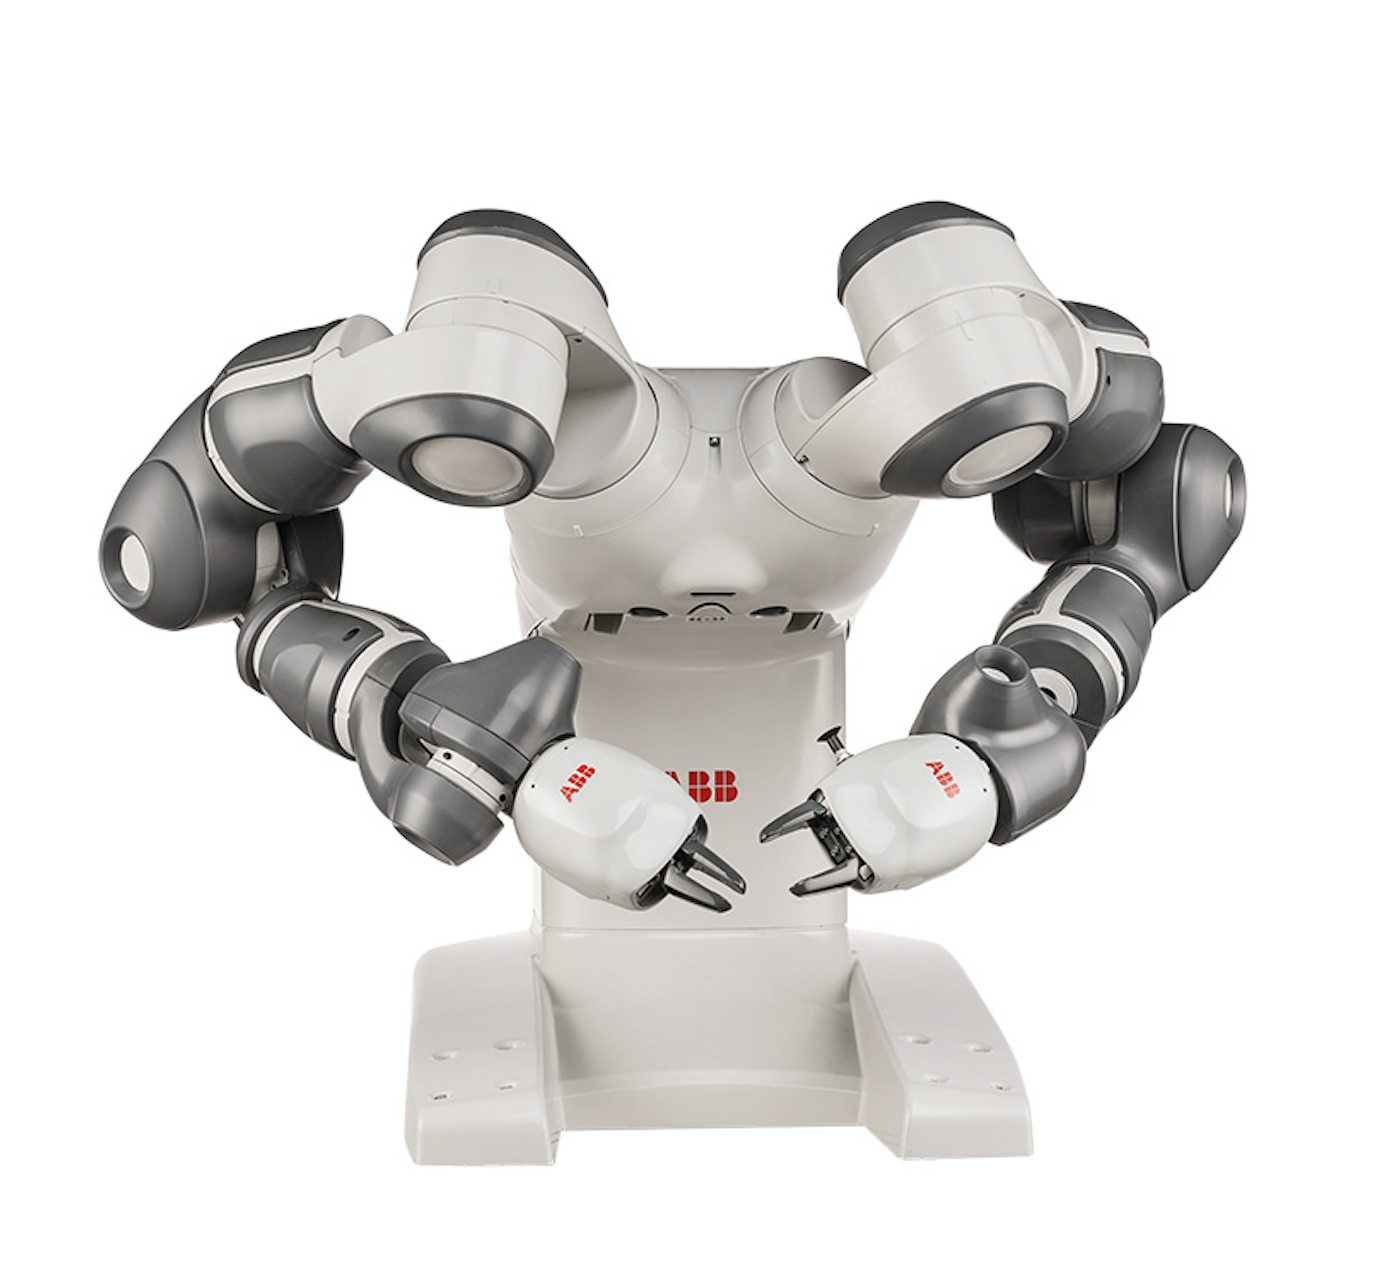
\includegraphics[width = 0.32\columnwidth]{background/YuMi.png}}
\caption{Three available robots}
\label{robot}
\end{figure}

The \citep{baxter} is a two-armed robot which is 3 feet tall and has a pedestal between 5'10" - 6'3" tall. Each of its arms has 7 degrees of freedom, whose movements are more reliable quicker than iCub. Baxter is usually used for simple industry jobs such as unloading, handling of materials. Considering its size, it is not suitable for this project. 

Referring to \citep{ABBsDual5:online}, YuMi is "a collaborative, dual arm, small parts assembly robot that includes flexible hands, parts feeding systems, camera-based part location and state-of-the-art robot control". With 7 degrees of freedom in each arm, it is designed for precise vision-based motion planning and thus is most appropriate to this project.

\section{Motion Planning} \label{backgroundmp}
The purpose of robotic motion planning is to seek the solution of the problem of "Go from the start configuration to the goal configuration while respecting all of the robot's constraints", such as avoiding collision with obstacles. A motion planning algorithm takes these tasks description as input, then calculates a path in configuration space. Below are several key concepts in robot motion planning problem.

\begin{itemize}
    \item \textbf{Work Space:} The physical space where the robot operates.
    \item \textbf{Configuration/State Space:} The configuration that describes the robot pose. For a solid 3D robot like YuMi, it can perform both 3D translation and 3D rotation. Therefore, a configuration needs six parameters: (x, y, z) for translation and (roll, pitch, yaw) for rotation, whose relationships are shown in Figure \ref{rpy}.
\end{itemize}

\begin{figure}[H]
\centering
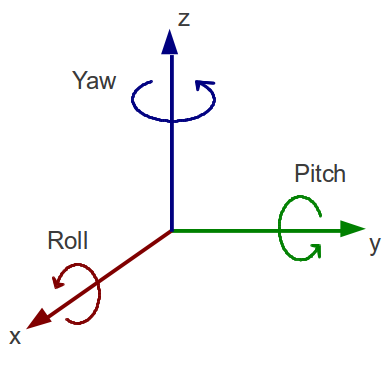
\includegraphics[width = 0.4\columnwidth]{background/rpy.png}
\caption{Roll, pitch, yaw rotation related to x, y, z axis}
\label{rpy}
\end{figure}

\begin{itemize}
    \item \textbf{Obstacle Space:} The space that robot cannot move to. 
    \item \textbf{Free Space:} The set of configurations of the robot that avoids collision with obstacles. To test if a configuration is in free space, forward kinematics will firstly be used to calculate the position of robot's geometry, and then collision detection will be performed to check if it collides with environment's geometry.
    \item \textbf{Target Space:} A subspace of free space that consists of interested positions we would like the robot to move to. In this project, the target space is determined by the camera.
    \item \textbf{Danger Space:} Space that robot is not desired but can move to. The robot usually passes through this space if the trajectory cannot be completed through free space.
\end{itemize}

According to \citep{OMPLPrim20:online}, there are plenty of methods still applicable in many scenarios, including exact and approximate cell decomposition, control-based methods, potential fields, and randomized planning. The summary of each method is as follow.

\begin{figure}[H]
\centering
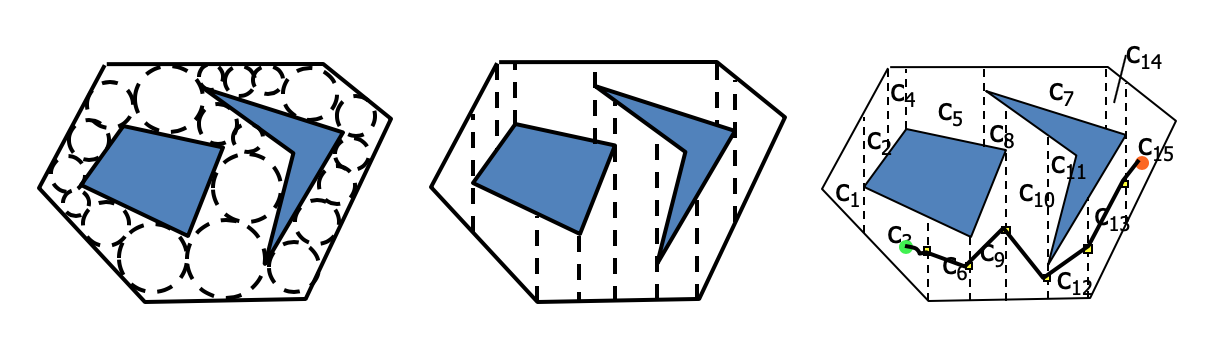
\includegraphics[width = \columnwidth]{background/cell.png}
\caption{2D cell decomposition example where the blue regions are obstacles \citep{celldecom}. From left to right: approximate cell decomposition, exact cell decomposition, and motion planning using exact cell decomposition. The available path is through C3, C6, C9, C10, C12, C13, and C15.}
\label{cell}
\end{figure}

\begin{itemize}
    \item \textbf{Exact and Approximate Cell Decomposition:} This approach partitions the workspace into discrete cells that corresponding to free space, where edges represent adjacency among cells and vertices indicate the individual cells (see Figure \ref{cell}). Therefore, the motion planning problem becomes a search from starting cell to the cell with the goal position. This method has a trade-off when setting the grid resolution. Coarser grid gives a faster search, but cannot find the path for narrow parts of free space. Moreover, the number of points on the grid is exponentially proportional to the configuration space dimension. This project has 6D state space, thus it is inappropriate to use this method.

    \item \textbf{Control-based Methods:} This method employs control theory and operates in continuous space. It typically uses feedback loops to manipulate the robot with minimal error. However, in complex dynamic environments, it is hard to calculate a feasible trajectory, and the valid motions will be restricted.

    \item \textbf{Potential Fields:} This technique computes a vector at each point in the workspace by summing an attractive force emanating from the goal, and a repulsive force from all obstacles and the boundaries (see Figure \ref{potentialexample}). It treats the configuration of the robot as a point in a potential field. Although it only requires little computation, navigating using gradient descent to follow the potentials to the goal can fail due to local minima in the field. This issue occurs when the attractive forces and repelling forces cancel each other out at a specific point.
\end{itemize}

\begin{figure}[H]
\centering
\subfigure[The potential field in a 2D space contains a goal and an obstacle \citep{potential}]{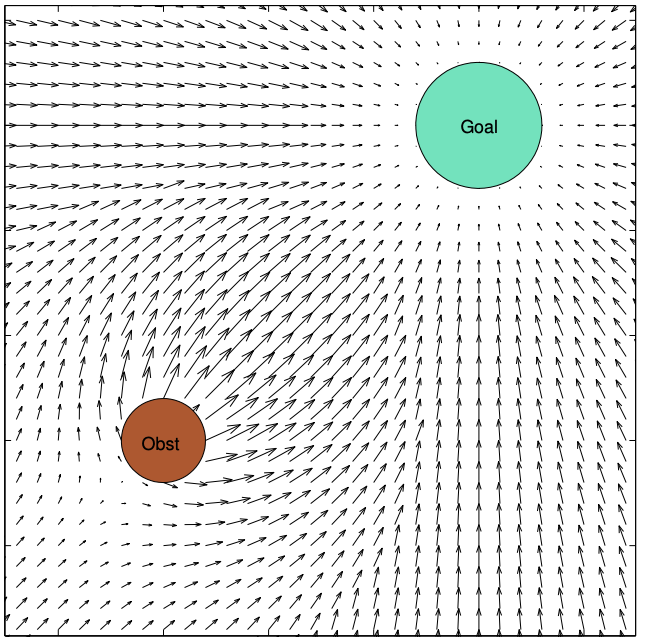
\includegraphics[height=5.3cm,keepaspectratio]{background/potentialfield.png}}
\subfigure[Potential field in 3D space \citep{3dpotential}. Warm colors represent high potential (obstacles), and cool colors indicate low potential (goals).]{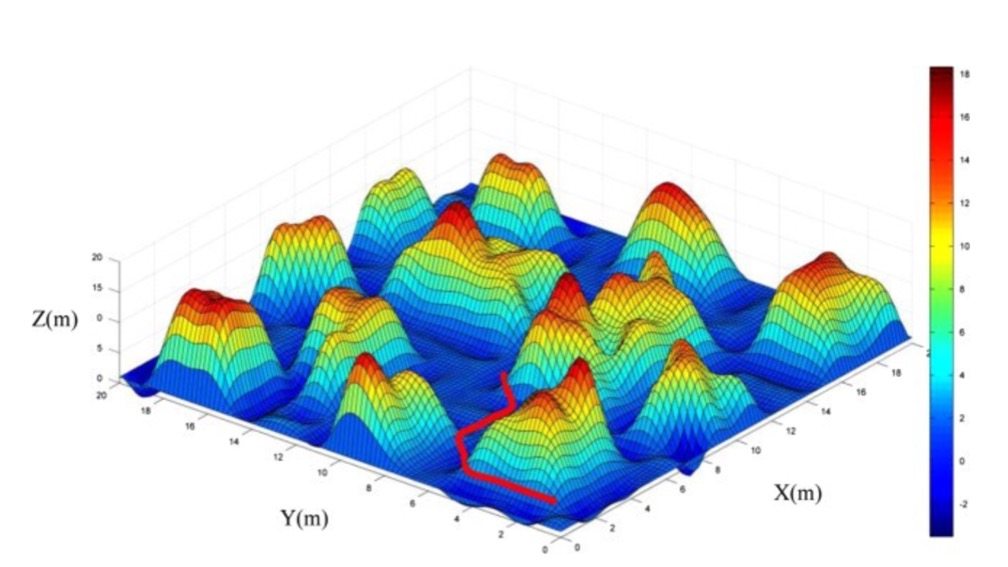
\includegraphics[height=5.3cm,keepaspectratio]{background/potentialfield3d.jpg}}
\caption{Example of the potential field approach}
\label{potentialexample}
\end{figure}

\begin{itemize}
    \item \textbf{Randomized Planning:} Randomization can be useful in motion planning. For example, in potential fields, it has been shown that Brownian motions where applying a random action for a specific amount of time can effectively guide a system out of the local minima.
\end{itemize}

The state-of-art sampling-based motion planning was inspired by randomization \citep{OMPLPrim20:online}, which employs sampling of the configuration space of the robot to answer planning queries effectively. It is especially suitable for systems with many degrees of freedom or differential constraints. Due to motion constraints and size of configuration space, traditional methods can spend a long time to address these problems. While sampling-based planning reasons over a finite set of configurations and connects these samples through collision-free paths. Usually, this method gives a probability to complete, as the number of samples reasoned increases, the possibility will converge to 1 if a solution exists. Nevertheless, it cannot determine if a problem does not have a solution, which can only be speculated by low probability. 

There are many existing sampling-based algorithms, such as Rapidly-expanding Random Trees \citep{RRT}, Probabilistic Roadmap Method \citep{Kavraki1996ProbabilisticRF}, Kinodynamic Planning by Interior-Exterior Cell Exploration \citep{Sucan2012AST} etc. Two typical planners are discussed below.

\begin{figure}[H]
\centering
\subfigure[The 2D work space and a single robot state]{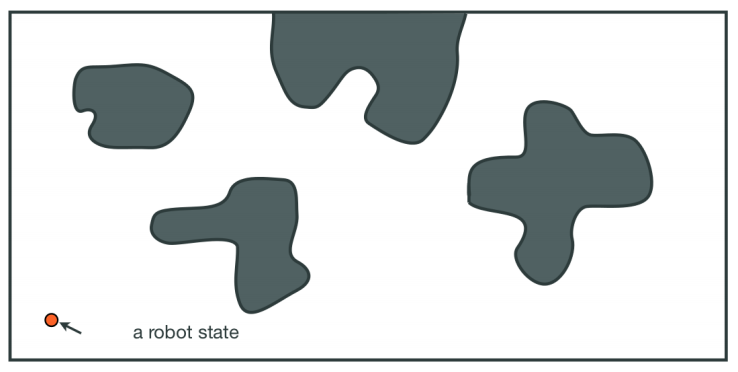
\includegraphics[width = 0.45\columnwidth]{background/rm1.png}}
\subfigure[One possible set of uniform random samples of free space]{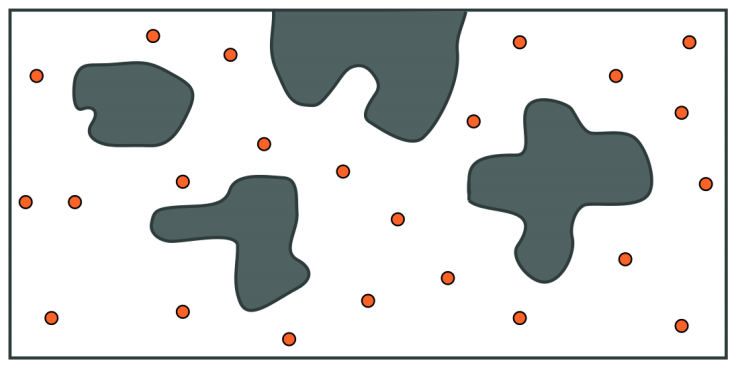
\includegraphics[width = 0.45\columnwidth]{background/rm2.png}}
\subfigure[PRM connects samples that are close to one another using a straight path in the free space]{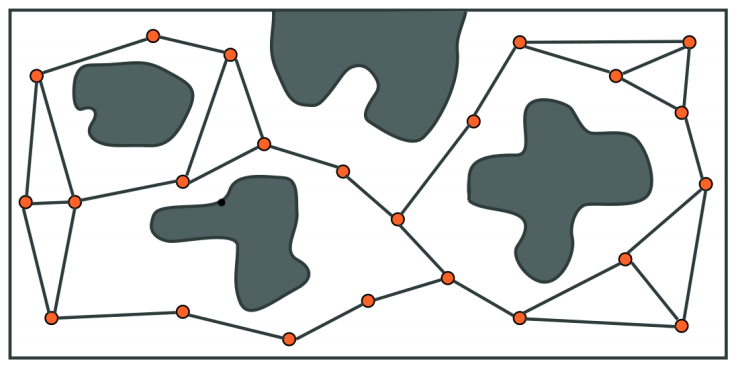
\includegraphics[width = 0.45\columnwidth]{background/rm3.png}}
\subfigure[The start and goal are connected to the roadmap, the shortest path is found]{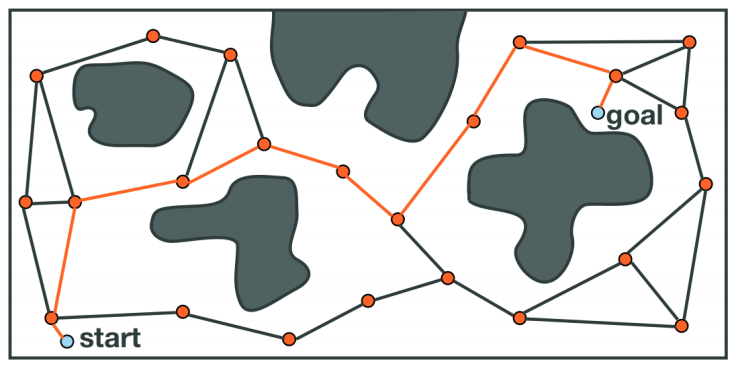
\includegraphics[width = 0.45\columnwidth]{background/rm4.png}}
\caption{Probabilistic roadmap example \citep{OMPLPrim20:online}}
\label{prm}
\end{figure}

\begin{itemize}
    \item \textbf{Probabilistic Roadmap (PRM)} \citep{Kavraki1996ProbabilisticRF}: The idea of this approach is to use random sampling of configuration space to construct a roadmap of free space. Figure \ref{prm} illustrates a simple example of PRM, where a 2D workspace and a point robot are used.
    
    The shaded areas represent obstacles. In sampling-based algorithms, free space usually cannot be known. As shown in Figure \ref{prm} (b), after performing the collision check, the collision-free samples are kept. Once sufficient free samples have been discovered, the roadmap will be built by connecting these samples. Utilizing a local planner whose task is to find a short collision-free path, each sample will be connected to its k nearest neighbors. Figure \ref{prm} (c) is the complete roadmap for this example. Finally, the start and goal states will be added to the roadmap, and a graph search can be fulfilled to compute the shortest path.
    
    \item \textbf{Tree-based Planners:} There are various types of tree-based planners (e.g. \citep{RRT}, \citep{Sucan2012AST}, \citep{inproceedings}, and \citep{hsu}). Here I will describe a general framework, as shown in Figure \ref{tree}. Notice that the biggest difference between tree-based techniques and PRM is that the former structure has no cycles.
    
    Starting from the start state, tree-based planners use random sampling to explore the next samples along a collision-free path expansively. Figure \ref{tree} (a) illustrates an example of first few valid samples. These planners usually bias their expansion towards the goal, if the existing tree can connect to the goal, then they complete the search. Figure \ref{tree} (b) is an example that the goal state cannot be directly connected to the tree, while \ref{tree} (c) shows the case where it can.
    
    Finally, because tree-based planners are directed and acyclic, they are more appropriate for single-query planning and complex dynamics.
\end{itemize}

\begin{figure}[H]
\centering
\subfigure[The first few random valid samples have been connected to the tree using an expansion heuristic]{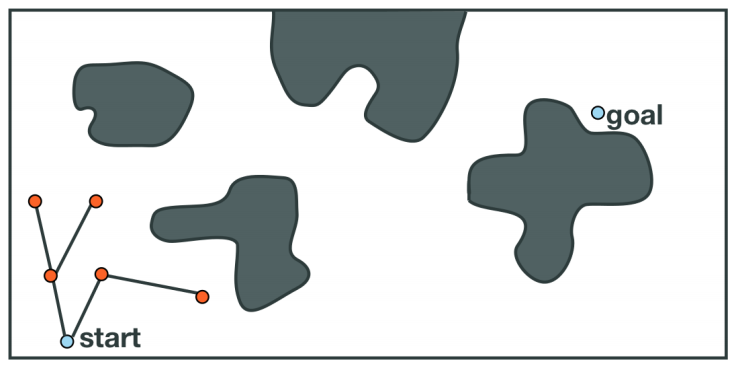
\includegraphics[width = 0.45\columnwidth]{background/rm5.png}}
\subfigure[Case when the goal cannot be connected to the tree because of an obstacle]{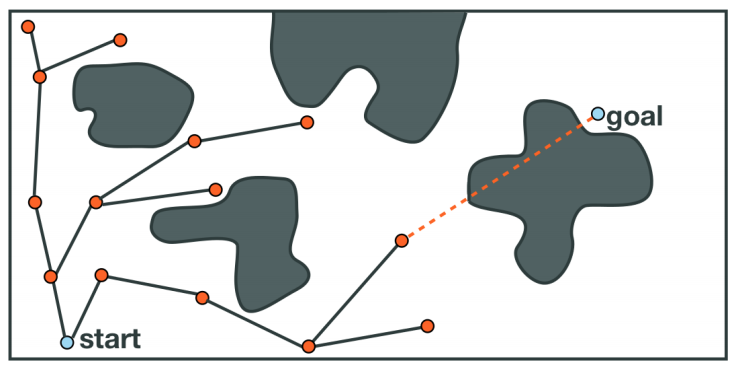
\includegraphics[width = 0.45\columnwidth]{background/rm6.png}}
\subfigure[Case when the goal can be connected to the tree]{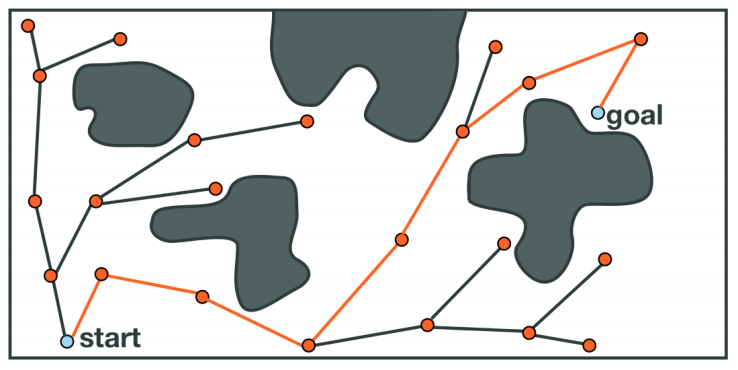
\includegraphics[width = 0.45\columnwidth]{background/rm7.png}}
\caption{Tree-based planners example \citep{OMPLPrim20:online}}
\label{tree}
\end{figure}

The memory requirement of sampling-based techniques is lower than other types of planners because no explicit representation of free configuration space is required. It is extremely powerful to plan in complex dynamics and high-dimensional space. However, generically implementing these algorithms is non-trivial. Thus, Open Motion Planning Library (OMPL) \citep{OMPL} is employed to plan the YuMi arm trajectories in this project, which is also available for use through the Robot Operating System (ROS).
In this case, after defining the configuration space, only start state, goal state, and environment scene needs to be supplied to plan a single motion. 

\section{Choice of Camera}
As mentioned in Section \ref{backgroundmp}, the configuration space for YuMi motion planning is 6D. Therefore, the state information, including 3D location and 3D orientation of the goal, must be provided before robot manipulation. In order to calculate the pose of shoe and shoelace, the camera needs to be able to provide depth information, which allows the user to segment images. 

In the beginning, there are two types of RGB-D cameras available in the Lab, ASUS Xtion PRO, and Microsoft Kinect. Both cameras provide similar functionalities, they all have an infrared emitter (left blue sensor), RGB camera (middle sensor), and an infrared depth camera (right sensor). Their resolutions are also the same, which is $640 \times 480$. Considering the ASUS Xtion PRO has already been fixed on the robot, I used it directly for algorithm development.

\begin{figure}[H]
\centering
\subfigure[ASUS Xtion PRO]{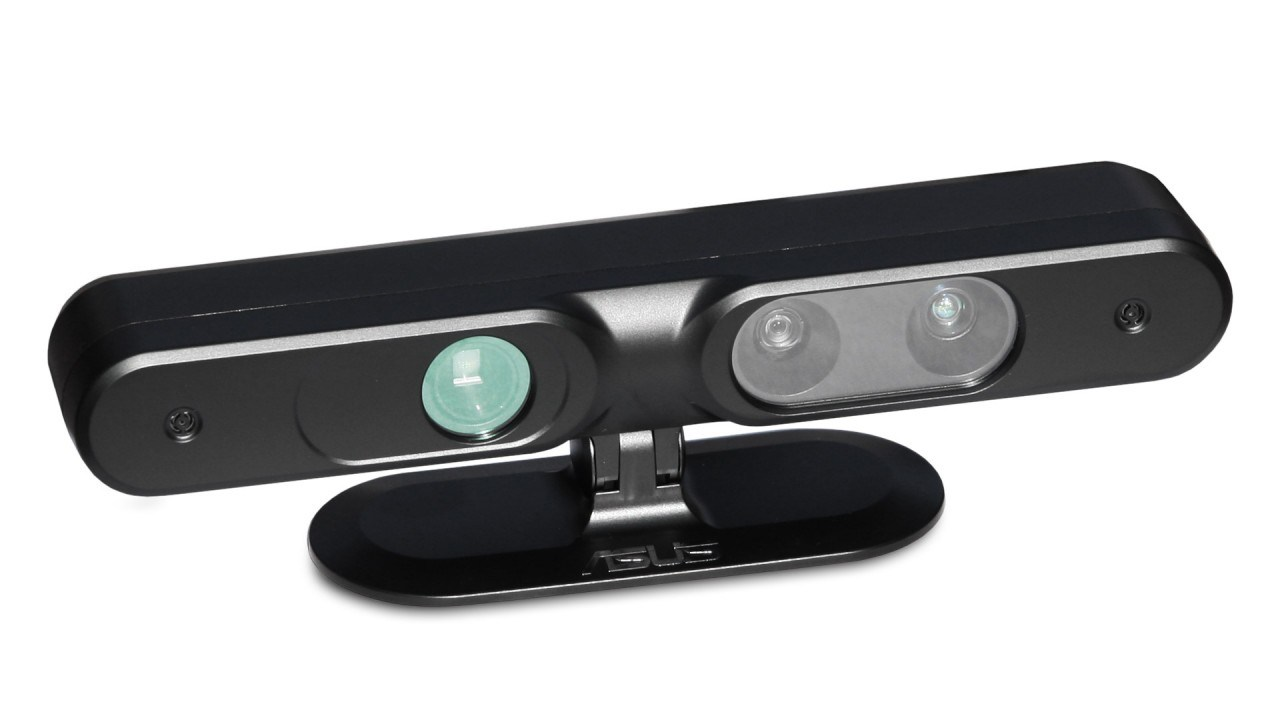
\includegraphics[width = 0.35\columnwidth]{background/asus.jpg}}
\subfigure[Microsoft Kinect]{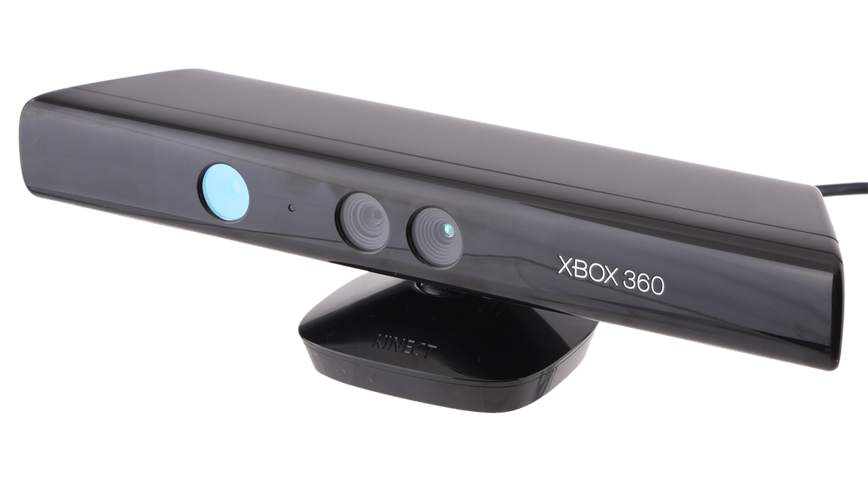
\includegraphics[width = 0.3\columnwidth]{background/kinect.png}}
\subfigure[ZED Mini]{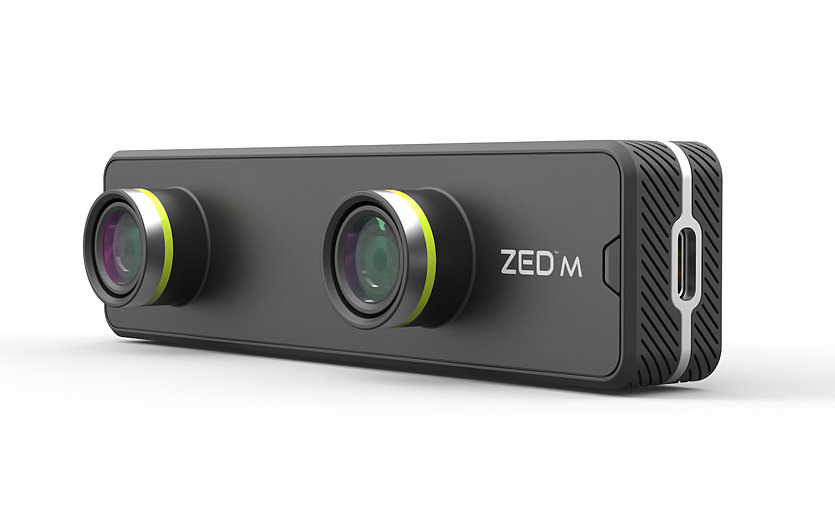
\includegraphics[width = 0.3\columnwidth]{background/zedmini.jpg}}
\caption{Three available cameras}
\label{camera}
\end{figure}

In the later stage of this project, another stereo camera named ZED Mini became available. It has two lenses with a separate film frame for each lens, which allows it to simulate human vision, and capture three-dimensional images. Its adjustable resolution is up to $2208 \times 1242$, much higher than that of ASUS Xtion and Kinect. Therefore, I ended up choosing this camera. It is worth mentioning that the final computer vision algorithms I implemented can be used on both ASUS Xtion and ZED Mini.


\section{Object Detection} \label{od}
Object detection is considered as one main part of computer vision, which can provide 2D positions of interested objects from an image. With the help of corresponding depth information provided by ASUS Xtion or ZED Mini, 3D location can then be determined. At present, there are several existing methods to detect the object's 2D pixel position.

A simple method to tackle this problem is by taking different target regions from the image and using CNN to classify the presence of the object within that area. However, since the number of occurrences of interested objects is not fixed, and they might have different spatial locations within the image and different aspect ratios, this approach could computationally blow up. Therefore, detection algorithms such as R-CNN \citep{RCNN}, YOLO \citep{YOLO} etc have been developed. 

The standard R-CNN method is not a complete end-to-end object detector and painfully slow. Fast R-CNN \citep{FastRCNN} improved the detection accuracy and speed, but the model relies on an external region proposal algorithm. With the propose of Faster R-CNN \citep{FasterRCNN}, R-CNNs became an end-to-end object detector which relies on a Region Proposal Network and removes the Selective Search requirement. The advantage of R-CNNs is their accuracy, but the biggest problem of them is their speed, obtaining only 5FPS on a CPU, which is unsuitable for real-time object detection. 

YOLO employs a one-stage detector strategy to increase the speed of deep learning based object detectors, which obtains 45FPS on a GPU. According to \citep{YOLO9000}, YOLO9000, which trained on both COCO detection dataset and ImageNet classification dataset, is capable of detecting over 9000 separate classes. Although it seems to be suitable for this project, shoelaces and shoe holes are not included in its detection range, and its accuracy needs to be tested. YOLOv3 \citep{YOLOv3} is the latest update of YOLO family. However, it is trained only on the COCO dataset that consists of 80 labels. The category of shoes is not included. Thus it is not suitable for this project. 

Another approach of detecting an object is color detection, which is available for this project. This is because the marked shoe which will be manipulated in this project has special shoelace and hole colors, which can be easily distinguished from the background. \citep{cie} converted RGB image to CIE-Lab color space to increase the accuracy of color segmentation. \citep{HSV} performed object segmentation using color filtering based on HSV (Hue, Saturation, Value) and calculated the centroid of the target. Although depth information can help discriminate objects that are not in the same plan as the object of interest, this method still has the disadvantage of been sensitive to the changes on lighting and is better being applied on the indoor environment. By carefully setting the color thresholds, this approach will be considered to use on shoe holes and shoelaces detection.

Shape detection is reckoned as an alternative way, which is achieved by segmenting point clouds and is suitable for detecting shoes. Furthermore, \citep{deformable_track} introduced an algorithm for tracking deformable objects form a sequence of point clouds, which is able to track a one-dimensional object such as ropes and shoelaces robustly. However, the method is not ready for public consumption right now and following the mathematics steps in the paper to programme is quite time-consuming.

\citep{vision_touch} presented an object-tracking framework that combines point cloud information from an RGB-D camera with GelSight contact sensor's tactile information. It also improves the pose accuracy during contact and provides robustness to occlusions of small objects. However, it is not suitable for YuMi robot.

Furthermore, OpenPose \citep{openpose} can jointly detect key points of the human body, hand, and foot, etc with high accuracy and reliability from images, which can also be a backup plan for shoe localization. One drawback of this approach is that people must wear the shoes in order for the algorithm to locate them, which will increase the complexity of experiments. Besides, letting robot manipulate the wearing shoes is considered to be complicated and unreliable because they can be shaken artificially.

According to these above research, this project will firstly employ YOLO9000 to detect shoes and use OpenCV color detection to identify holes and laces. Based on their performances, other approaches will be considered whether to be applied or not.

\section{Orientation Estimation} \label{oriestimation}
To provide the complete state information to the robot, the 3D orientation of the interested object needs to be calculated besides its 3D location that is discussed in Section \ref{od}. In this project, particularly, the orientation of shoe holes has to be computed so that the shoelace can be successfully put into them.

There are several existing state-of-the-art 6D object pose estimation methods. \citep{singleshot} proposed a real-time single-shot approach to predict the object's 6D pose, which does not require additional post-processing. They first employed CNN to compute 2D image locations of projected vertices of the object's 3D bounding box. Then a PnP algorithm is utilized to estimated 6D pose. However, these kinds of methods become unreliable when low-texture or low-resolution inputs are given. \citep{PoseCNN} introduced PoseCNN, estimates the object's 3D rotation by regressing to a quaternion representation using only color images. They also presented a novel loss function to let PoseCNN handle symmetric objects. Depth data is used for further refinement. \citep{DeepIM} presented DeepIM, given an initial pose estimation, it can refine the object's pose by matching the rendered image against the observed image iteratively. DeepIM only uses color images to introduce the untangled pose representation, which is independent of the 3D object model's coordinate frame and the object size. \citep{DenseFusion} proposed DenseFusion, which processes both color and depth information separately and employs a dense fusion network to extract pixel-wise dense feature embedding, from which the pose of known objects can be predicted. Moreover, it is robust against occlusions and outperforms PoseCNN after refinement on two benchmarks for 6D pose estimation, YCB-Video \citep{PoseCNN} and LineMOD \citep{linemod} respectively.

However, these algorithms only compute object pose, after retraining them using shoe dataset, which needs to be prepared by myself. Besides, they cannot calculate the orientation of a specific region on the interested object, such as shoe holes'. In order to achieve this function, the 6D pose correlations of shoe holes and centroid of shoe need to be determined. After that, once these algorithms compute shoe pose, the pose of holes can be determined accordingly. Nevertheless, calculating these correlations are difficult and time-consuming. Moreover, once the shoe is squeezed and deformed, these relationships have to be defined again. Therefore, based on these considerations, those 6D pose estimation approaches cannot be my first choice.

To tackle this problem, another method I came up with is inspired by Random Sample Consensus (RANSAC) \citep{rsc}. RANSAC can estimate parameters of a mathematical model from a set of data containing both inliers and outliers. It selects a random subset of the original data interactively to form hypothetical inliers and then tests this hypothesis as follows:

\begin{enumerate}
    \item Fit a model to the hypothetical inliers.
    \item Test the fitted model using all other data. If there is a good fit between a data and the estimated model, then this data will be regarded as a hypothetical inlier.
    \item If there are sufficient data be considered as hypothetical inliers, the computed model is good.
    \item Re-estimate the model using all hypothetical inliers.
    \item Evaluate the model by estimating the error of the model related to the inliers.
\end{enumerate}

Each time of this procedure will produce a refined model with a corresponding error or a model that is rejected because only a few data are classified as inliers. In the former case, the refined model will be kept if its error is lower than the last saved model.

\begin{figure}[H]
\centering
\subfigure[A dataset containing both inliers and outliers]{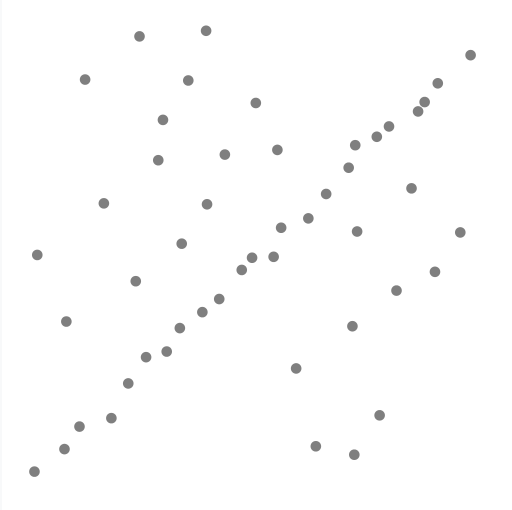
\includegraphics[width = 0.45\columnwidth]{background/rsc1.png}}
\subfigure[Using RANSAC to compute the best fitting line. Blue points represent inliers, red points are outliers]{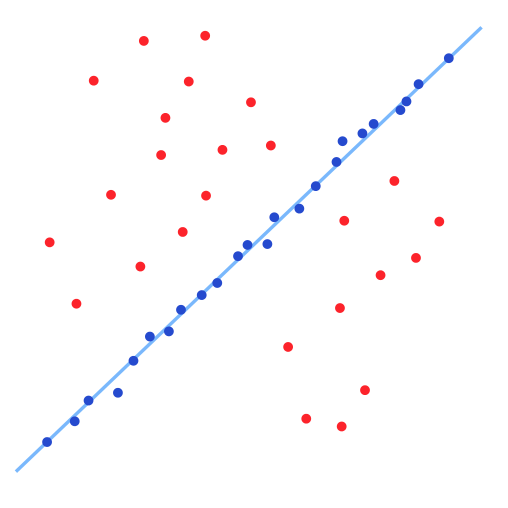
\includegraphics[width = 0.45\columnwidth]{background/rsc2.png}}
\caption{RANSAC example \citep{random}}
\label{ransac}
\end{figure}

RANSAC can estimate the model parameters accurately, even if the number of outliers is large. , and thus, there is a trade-off between time and accuracy. Furthermore, the problem-specific thresholds need to be set as well. Figure \ref{ransac} is the example of applying RANSAC on the 2D dataset to estimate a best fitting line.

For this project, the orientation of a shoe hole can be represented as the normal vector of its surrounding area. The method I introduce is by applying RANSAC technique to construct a plane of interested shoe hole, then computing the normal vector accordingly. Moreover, with the help of some pre-defined constraints and data processing techniques, the accuracy and robustness of resulting orientation can be further improved.

\section{System and Software}
All programs of this project will run under Ubuntu system. ROS will act as the middleware between YuMi and the software, which creates a network of Nodes in order to control different functionalities of the robot. By sending messages from one Node to others, communication can be achieved between Nodes. To be specific, the sender advertises on a given topic, while the receiver subscribes that corresponding topic. After compiling a standalone program into a ROS package, it is able to run on the ROS network. In addition, these programs need to be written in Python or C++.

Apart from that, MoveIt! will be used to provide motion planning functionality in ROS, which can load robots' URDF file and create appropriate state spaces for user-defined joint groups and call OMPL planners to find feasible paths. MoveIt! then translates the path produced by OMPL into dynamically feasible trajectories. Self-collisions can also be discovered on a pre-processing phase by MoveIt!.
\chapter{Requirements Capture}
%ability independently to formulate and solve technical problems in project work. 
%The project specification should state clearly what the project is intended to deliver, including all hardware, software, simulation.

\section{The Project Deliverable}
The objective of this project is to solve of problem of putting shoe laces on a shoe using bi-manual robot YuMi. Starting with one arm holding the shoelace, YuMi should detect a shoe hole and pass the shoelace through it by planning an arm trajectory. For more challenging ...

\begin{figure}[H]
\centering

\includegraphics[width = 0.5\columnwidth]{images/ph.png}
\caption{The manipulated shoe with distinct lace and hole colors}
\label{shoe}
\end{figure}

To constrain the problem, a shoe with distinct lace and hole colors will be used as the target for manipulation, which is shown in Figure \ref{shoe}. In addition, the entire manipulation process will be carried out on the workbench of the Imperial College Personal Robotics Lab under normal lighting condition.

The core project deliverable can be divided into two main parts: Computer Vision and Motion Planning.

\section{Computer Vision}
This part aims to compute the real-time 6D pose of a specific shoe hole. The algorithm must provide an accurate and stable result so that it can be used for actual shoe lace manipulation. The following features should be delivered:

\begin{itemize}
    \item \textbf{Shoe Detection:} Detecting the 2D location of the shoe when it is placing on the workbench.
    \item \textbf{Shoe Hole Tracking:} Detecting the 2D position of interested shoe hole and its contour area
    \item \textbf{3D Location Estimation:} Computing the 3D location of the centroid of that hole
    \item \textbf{3D Orientation Estimation:} Computing the 3D orientation of that hole
    %\item \textbf{Shoelace Localization:}
\end{itemize}


\section{Motion Planning}
This part focus on real-world motion planning of YuMi's arms. The outcome of this part should enable YuMi to put shoe lace into a hole accurately while avoiding any collisions with obstacles. Once finishing, both arms should return to their default poses. Following tasks must be completed:

\begin{itemize}
    \item \textbf{Movement Control:} Setting up the control interface among my control instructions, MoveIt! and YuMi.
    \item \textbf{Planning Scene Setup:} Initializing the manipulating environment, defining obstacles' dimension and position.
    \item \textbf{Safety Positions Calculation:} Calculating several safety poses of YuMi's arms, including default poses, initial poses etc.
    \item \textbf{Shoe Pose Adjustment:}
    \item \textbf{Robot Gripper Approaching Pose:} Computing the 6D approaching pose to the interested shoe hole.
    \item \textbf{Offset Adjustment:} Adjusting the offset between camera readings and YuMi movement, especially its influence on gripper's pose.
    %\item \textbf{Shoelace Grabbing:}
\end{itemize}



%\section{Testing Environment}
%light pose robot .....

% The central part of the report usually consists of three or four chapters detailing the technical work undertaken during the project. 
\chapter{Analysis and Design}

\section{ROS and YuMi Overview}
As discussed in the Background Chapter, ROS handles a number of independent Nodes that performs specific function(s). They communicate with each other by publishing messages to topics or subscribing them. ROS messages support several data formats, including number, string, and time etc. Moreover, these communications are only available if a $roscore$ is running, which is a collection of programs and Nodes that are prerequisites of a ROS-based system.

Besides, $TF$ is an important package in ROS and used several times in this project. According to \citep{tfROSWik}, it maintains the relationship between coordinate frames (such as camera frame, robot fram etc.) in a tree structure buffered, which enables the user to transform points, vectors, etc between any two coordinate frames at any desired point in time. Details will be discussed in Implementation Chapter.

The dual-arm robot YuMi communicates with ROS using Personal Robotics Lab setup (User Guide Chapter contains more details). YuMi has one gripper camera embedded in each of its gripper. Using these cameras may provide more accurate results of shoe and shoe hole locations. However, in order to use these two cameras, a package named $abb\_rws\_interface$ which is a proprietary interface of ABB is required. According to \citep{EGMfiles}, it is not public. Also, the open source version of that package called $abb\_librws$ cannot match the current $yumi\_cameras$ setup. Furthermore, it is not very feasible to tie a small camera to YuMi's arms. Therefore, this project will only utilize the ASUS Xtion camera for detection.

\section{System Overview}

\begin{figure}[H]
\centering
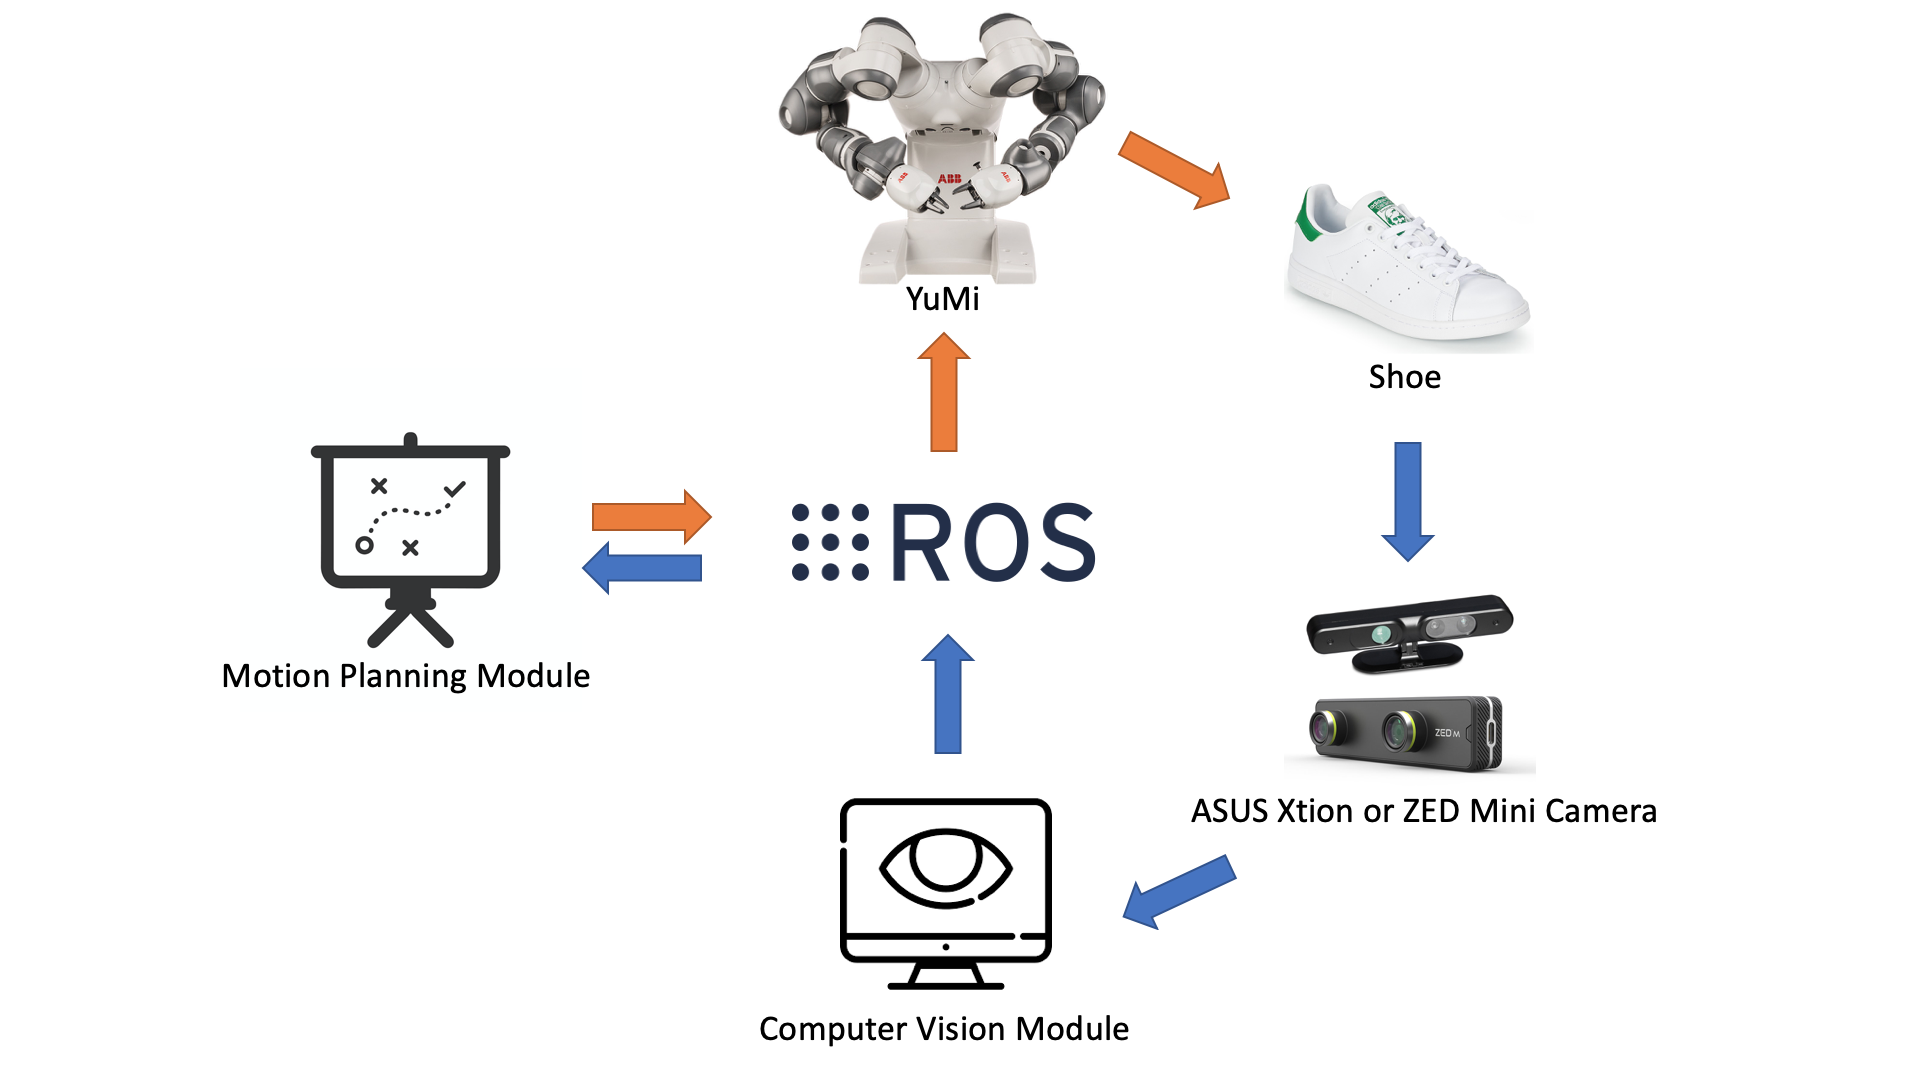
\includegraphics[width = \columnwidth]{AnalysisDesign/system.png}
\caption{System overview}
\label{c4}
\end{figure}

Figure \ref{c4} displays the system overview of this project, which consists six components: the shoe, ASUS Xtion camera, computer vision module, ROS Kinetic, motion planning module, and YuMi. Blue arrows represent computer vision messages and orange arrows indicate related motion plans and manipulation.

Starting from the camera, which consistently recording RGB and depth images of the workbench and outputs them to the computer vision module. The module then performs several functions including shoe detection, shoe hole tracking, 6D shoe hole pose estimation etc. and publishes the corresponding message to ROS topics. After that, the motion planning module subscribes these information and plans YuMi arms trajectories accordingly to adjust shoe pose or put lace on a hole. If the planning succeeds, YuMi will then execute these motions to manipulate shoe and shoe lace.

The following two chapters will discuss detailed implementation approaches.
%detail---------------------------
\chapter{Implementation}

\section{ROS and YuMi Overview}

\section{Camera..}

\section{Shoe Detection}

%\section{Shoe Position Adjustment}

\section{Shoehole Tracking}

\section{Angle of Approach}

\section{Pose Estimation}

\section{Offset Adjustment}

%\section{Stage Two...}
\chapter{Testing}

\section{Detection}

\section{Motion Planning}
\chapter{Results}
\chapter{Evaluation}
\chapter{Conclusion}

This project successfully addressed the precise AI planning and control problem - putting a shoelace on a shoe using bimanual robot, YuMi, and an external camera. All the specified requirements were met.

\begin{figure}[H]
\centering
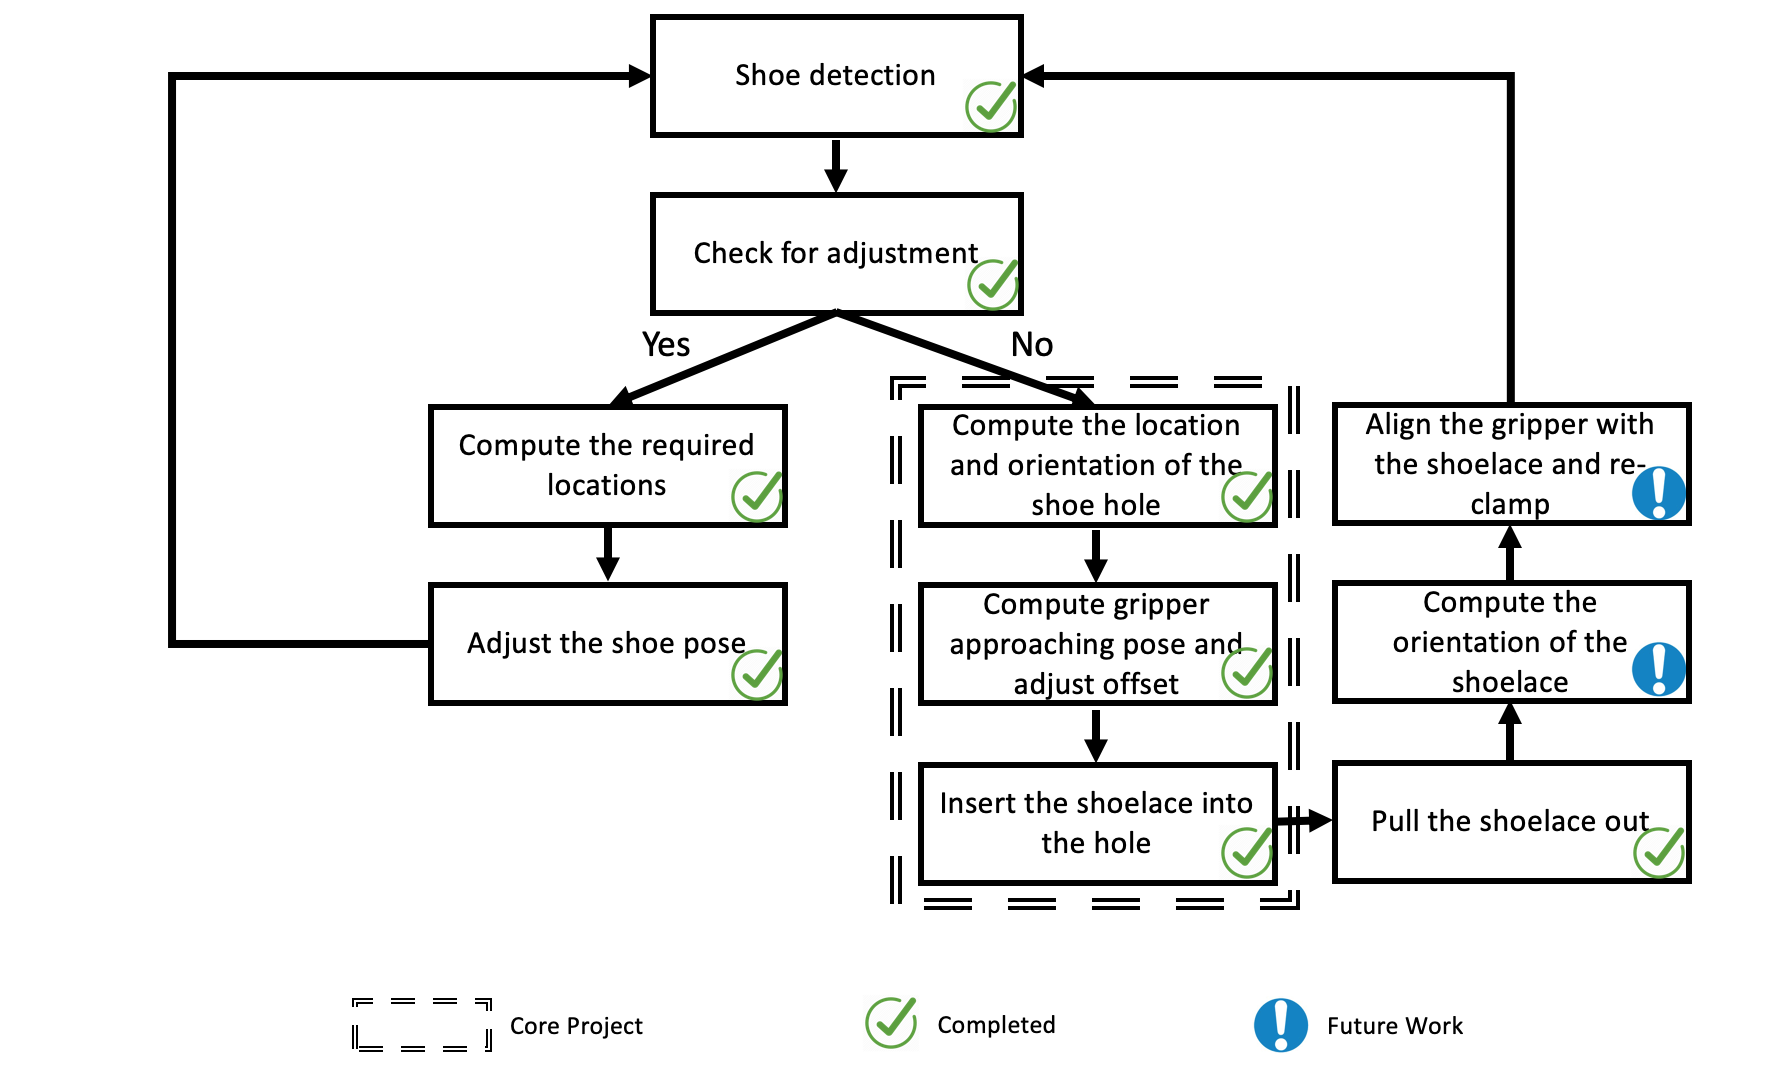
\includegraphics[width = \columnwidth]{conclusion/workflowcon.png}
\caption{The project achievements}
\label{workflowcon}
\end{figure}

Recall the system workflow, as shown in Figure \ref{workflowcon}, the core project which is passing the shoelace into a hole has been successfully completed. Besides, YuMi equips with capabilities to adjust the pose of the shoe if necessary, as well as grab and pull the shoelace out to a proper location for further manipulation after insertion. The corresponding success rates with deal with shoe hole with $4mm$ radius can be found in Table \ref{sris}, which are calculated based on the results shown in Figure \ref{integratedtest}.

\begin{table}[H]
\centering
\begin{tabular}{||c|c|c|c||}
\hline
Detection & Adjustment & Insertion & Pulling \\ \hline\hline
100\% & 95\% & 87\% & 91\% \\ \hline
\end{tabular}
\caption{The success rate of integrated system}
\label{sris}
\end{table}

For computer vision part, the two cameras, ASUS Xtion and ZED Mini, were correctly set up and calibrated. All computer vision algorithms in this project were implemented for both of them. As discussed in Section \ref{shoedetection}, the shoe can be successfully detected by employing YOLO, regardless of whether there are other interfering objects on the workbench. The calculation of required locations for shoe pose adjustment is introduced in Section \ref{shoeadjust}. All location conversions between camera frame and YuMi frame in this project are based on ROS $TF$ topic. Real-time 6D pose (3D location and 3D orientation) of shoe hole can also be estimated with high precision by utilizing techniques introduced in this report. The location is calculated based on some image processing techniques including color detection, blurred filters etc, details can be found in Section \ref{3dlocationestimation}. Moreover, I extracted the region of shoe and carefully set the color thresholds in advance to further reducing the impact of lighting conditions on the results. The method to compute accurate orientation of the shoe hole is mentioned in Section \ref{3DOrientationofShoeHole}, which is based on RANSAC. The orientation had great volatility, especially when using the low-resolution camera such as ASUS Xtion. Therefore, I introduced some pre-defined constraints to tackle this issue and finally averaged out the valid readings within a certain time.

For motion planning part, my algorithms can successfully plan and move YuMi for shoe and shoelace manipulation while avoiding potential collisions with the environments. The important details about interface and planning scene setup are told in Section \ref{motionplansetup}. The movement control, and related implementation methods such as setting joint goals and pose goals are discussed in Section \ref{movementcontrol}. The three safe poses throughout manipulation process are defined in Section \ref{safetyposescalculation}. Detailed shoe pose adjustment plan, shoelace insertion plan, shoelace grabbing and pulling plan and a series of their movement photo examples can be found in Section \ref{adj}, \ref{approachposegripper}, and \ref{shoelacegrabbing} respectively. Each plan contains several preparation postures and retreat postures. Both single-arm motion planning and dual-arm coordination are implemented. The accurate offset adjustment approach is in Section \ref{offsetadjustment}.

The advantages of the final integrated system are fast, relatively stable, and only require one camera. The qualitative and quantitative results can be found in Testing and Results Chapter, which proves that YuMi can completely overcome shoelace insertion challenge for $7.5mm$ radius shoe hole (100\% success rate) and .

However, for my approach, the precision of 6D pose of shoe hole largely depends on the resolution of the camera. In addition, the offset needs to be adjusted every time the relative pose between the camera and the robot changes. These issues can be resolved by using the YuMi gripper camera, however it is currently unavailable. An alternative is to find an appropriate way to attach another small camera to YuMi's arm. By doing this, YuMi can adjust its gripper pose referenced to the pose of interested shoe hole continuously through the image feedback from the wrist camera. The accuracy is considered to be improved while the operation will become slower. More details are included in Section \ref{futurecamera}.


%A series of experiments have validated the proposed method, highlighting its strengths and drawbacks, but ultimately demonstrating high performance and versatility. The learning method was heavily inspired by combinations of previous works, but also introduced some novel techniques which contributed to the overall robustness of the system.

To complete the project extension, the last two parts in Figure \ref{workflowcon} workflow: "compute the orientation of the shoelace" and "align the gripper with the shoelace and reclamp" have to be implemented. The methods are no different from what have been described in the report. The former can be achieved by using color detection and RANSAC. Similarly, YuMi can align its right gripper with the colored head of shoelace and accomplish reclamping according to the approaches introduced in Section \ref{approachposegripper}. Adjusting shoe pose using single arm can refer to Section \ref{adj}. After that, the whole workflow is completed and the shoelace can be passed into every hole of the shoe.

Finally, there are some initial definitions for this project, such as the shoe and shoelace are marked, the shoelace is held by YuMi before insertion etc. Discussion about how to completely solve the problem of putting normal shoelace on a regular shoe can be found in the next chapter. 


%critical evaluation compare to previous ....product, algorithm, ...
 %- design choice 
 %- what did I learn
%advantages (positively and worthwhile) achievement!!

\chapter{Future Work}

\section{Construction Shoe Model}
\section{Deformable Object Tracking}
\section{Gripper Camera}
\section{Reinforcement Learning}
\chapter{User Guide}
This guide aims to support anyone who would like to use the delivered system or continue this project. The Github repository is \url{https://github.com/Martinpanzy/FYP-Yumi}.

\section{Dependencies}
%install/ configure/ use
\section{ROS Packages}

\section{Usage}

%\section{Code}
%do not put full code, it will be seen as padding up the thesis for no reason. Point to a GitHub directory, and put in here maybe pseudocode, or configuration file specifications etc. 


\bibliographystyle{plainnat}
\bibliography{bibs/sample}
\appendix
\chapter{First Appendix}
%Self-propelled arrangement of and conduct at project meetings. 
%Setting agendas and work plans. 
%Ownership of project specification and development of objectives. 
%Appropriate self-driven use of supervisor (or other people) as source of information and advice.

%Information typically included are things like program listings, complex circuit diagrams, tables, proofs, graphs or any other material which would break up the theme of the text if it appeared in situ.

%\chapter{Issues}

\section{Safety}
There are some foreseeable safety risks of this project, each of which is listed below and the corresponding solution is discussed. 

\begin{itemize}
 \item Electrical safety - shocks to myself or others from YuMi power supply.

Solution: Carefully plug-in power supply to YuMi each time and follow the instruction manual to turn on and shut down. 

 \item Physical safety - damage from YuMi's arms and grippers to me and others.
 
Solution: YuMi is placed in a spacious environment, whose arm and gripper could not enter lab members' normal range of activities. Moreover, according to YuMi's product specification \citep{Productspecification}, if an unexpected mechanical disturbance happens, the robot will stop and then slightly back off from its stop position. In addition, YuMi's Cartesian speed supervision function limits its elbow and wrist speed in both manual and automatic mode. Once the limit is exceeded, the robot motion will be stopped. Finally, the FlexPendant emergency stop button can remove power from the actuators thus stop the robot. 
 
 \item Fire safety - possible fire risk from YuMi.

Solution: YuMi removes the batteries thus eliminate the fire risk when charging. Also, the robot system complies with the requirements of UL (Underwriters Laboratories) for fire safety \citep{Productspecification}.

 \item Data Infrastructure safety
 
Solution: One laptop from Imperial College Personal Robotics Lab will be used in this project. I am using a separate user account thus will not adversely affect other people's code or programs.
 
\end{itemize}

In general, any operations that I am uncertain about whether it will cause a safety issue will be made after asking the PhDs in the lab. 

\section{Ethical}
As the development of robotics, there are more and more ethical and social implications posed by this technology need to be aware of. Some typical issues include job displacement, privacy, AI bias etc. Considering this project, machine learning might not be applied to motion planning part and the vision algorithm is based on the open source YOLO and OpenCV libraries. The real-time images obtained from cameras will not be saved or used except to lace up shoes. The robot will not draw on information about the user’s current physical, cognitive and emotional state etc, thus it is reckoned that the privacy and AI bias issues are not the concern. The aim of this project is robotics research. Thus, it is not considered that the progress of this project will be used in an industrial company and replace human. 

\section{Legal}
The code of this project will mainly be developed by myself and only will employ some open source libraries such as OpenCV and OMPL etc. Therefore will not infringe the intellectual property rights of others.

\end{document}